\def\duedate{09/29/22}
\def\HWnum{1}
% Document setup
\documentclass[12pt]{article}
\usepackage[margin=1in]{geometry}
\usepackage{fancyhdr}
\usepackage{lastpage}

\pagestyle{fancy}
\lhead{Richard Whitehill}
\chead{PHYS 714 -- HW \HWnum}
\rhead{\duedate}
\cfoot{\thepage \hspace{1pt} of \pageref{LastPage}}

% Encoding
\usepackage[utf8]{inputenc}
\usepackage[T1]{fontenc}

% Math/Physics Packages
\usepackage{amsmath}
\usepackage{amssymb}
\usepackage{dsfont}
\usepackage{mathtools}
\usepackage[arrowdel]{physics}
\usepackage{siunitx}

\AtBeginDocument{\RenewCommandCopy\qty\SI}

% Reference Style
\usepackage{hyperref}
\hypersetup{
    colorlinks=true,
    linkcolor=blue,
    filecolor=magenta,
    urlcolor=cyan,
    citecolor=green
}

\newcommand{\eref}[1]{Eq.~(\ref{eq:#1})}
\newcommand{\erefs}[2]{Eqs.~(\ref{eq:#1})--(\ref{eq:#2})}

\newcommand{\fref}[1]{Fig.~\ref{fig:#1}}
\newcommand{\frefs}[2]{Figs.~\ref{fig:#1}--\ref{fig:#2}}

\newcommand{\tref}[1]{Table~\ref{tab:#1}}
\newcommand{\trefs}[2]{Tables~\ref{tab:#1}-\ref{tab:#2}}

% Figures and Tables 
\usepackage{graphicx}
\usepackage{float}

\newcommand{\bef}{\begin{figure}[h!]\begin{center}}
\newcommand{\eef}{\end{center}\end{figure}}

\newcommand{\bet}{\begin{table}[h!]\begin{center}}
\newcommand{\eet}{\end{center}\end{table}}

% tikz
\usepackage{tikz}
\usetikzlibrary{calc}
\usetikzlibrary{decorations.pathmorphing}
\usetikzlibrary{decorations.markings}
\usetikzlibrary{arrows.meta}
\usetikzlibrary{positioning}

% tcolorbox
\usepackage[most]{tcolorbox}
\usepackage{xcolor}
\usepackage{xifthen}
\usepackage{parskip}

\newcommand*{\eqbox}{\tcboxmath[
    enhanced,
    colback=black!10!white,
    colframe=black,
    sharp corners,
    size=fbox,
    boxsep=8pt,
    boxrule=1pt
]}

% Miscellaneous Definitions/Settings
\newcommand{\prob}[2]{\textbf{#1)} #2}

\setlength{\parskip}{\baselineskip}
\setlength{\parindent}{0pt}

\def\complexs{\mathbb{C}}
\def\reals{\mathbb{R}}
\def\naturals{\mathbb{N}}
\def\integers{\mathbb{Z}}
\def\rationals{\mathbb{Q}}
\def\id{\mathds{1}}



\setlength{\headheight}{14.9998pt}
\addtolength{\topmargin}{-2.49998pt}

\begin{document}
    
\prob{1}{
Assume $x$ is an $m$-dimensional vector, prove $||x||_{\infty} \leq ||x||_{2}$ and $||x||_{2} \leq \sqrt{m} ||x||_{\infty}$.
}

Recall that 
\begin{align}
    \label{eq:norm-def}
    ||x||_{2} &= \sqrt{\sum_{i=1}^{m} |x_{i}|^{2}} \\
    ||x||_{\infty} &= \max \{ |x_1|,|x_2|, \ldots, |x_{m}| \} 
.\end{align}

Thus, for the first inequality we have the following.
Suppose that $|x_{k}| = ||x||_{\infty}$, then
\begin{eqnarray}
    \label{eq:derive-1st-inequality}
    \eqbox{
    ||x||_{2} = \sqrt{||x||_{\infty}^2 + \sum_{i \ne k} |x_{i}|^2} \leq \sqrt{||x||_{\infty}^2} \leq ||x||_{\infty}
}
,\end{eqnarray}
since $|x_{i}| \geq 0$ for all $i$.

For the second inequality, we know that $|x_{i}| \leq ||x||_{\infty}$ for all $i$.
Hence,
\begin{eqnarray}
    \label{eq:derive-2nd-inequality}
    \eqbox{
    ||x||_{2} \leq \sqrt{\sum_{i=1}^{m} ||x||_{\infty}^2} = \sqrt{m}||x||_{\infty} 
}
.\end{eqnarray}



\prob{2}{
Show that if a matrix $A$ is both triangular and unitary, then it is diagonal.
}

Suppose that $A = (a_{ij}) \in \complexs^{n \times n}$ is an upper triangular matrix we know that $a_{ij} = 0$ if $i > j$.
First, we will show that $A^{-1}$, assuming that $A$ is non-singular, is upper triangular.
Let $A^{-1} = [b_1 b_2 \ldots b_{n}]$, then $A^{-1}A = \id$ and
\begin{eqnarray}
    \label{eq:inverse-equations}
    \begin{cases}
    b_1a_{11} = e_1 \\
    b_2a_{12} + b_2a_{22} = e_2 \\
    \vdots \\
    b_1a_{1n} + b_2a_{2n} + \ldots + b_{n}a_{nn} = e_{n}
    ,\end{cases} 
\end{eqnarray}
where $(e_{i})_{j} = \delta_{ij} = \begin{cases}
    1 & i = j \\
    0 & i \ne j
\end{cases}$
is the standard basis.
From lectures, we know that we can solve this system using forward substitution as follows:
\begin{eqnarray}
    \label{eq:backsub}
    \begin{cases}
    b_1 = e_1/a_{11} \\
    b_{i} = (e_{i} - \sum_{k=1}^{i-1} b_{k}a_{ki})/a_{ii}
    .\end{cases} 
\end{eqnarray}
Observe that
\begin{align}
    \label{eq:prove-upper-triangle}
    (b_1)_{j} &= \frac{1}{a_{11}}\delta_{1j} \\
    (b_{i})_{j} &= \frac{1}{a_{ii}}\delta_{ij} - \sum_{k=1}^{i-1} (b_{k})_{j}\frac{a_{ki}}{a_{ii}}
.\end{align}
Using induction, it is easy to see that $b_{ij} = 0$ if $i > j$.

Next, we will show that $A^{\rm T}$ must be lower triangular, which implies that $A^{\dagger} = A^{* {\rm T}}$ is lower triangular.
From the definition $(A^{\rm T})_{ij} = a_{ji}$.
Since $a_{ji} = 0$ if $j > i$, then it follows that $(A^{\rm T})_{ij} = 0$ if $j > i$, which proves that $A^{\rm T}$ is lower triangular.

Now, let $A$ be a unitary.
Then, $A^{\dagger} = A^{-1}$.
Hence,
\begin{eqnarray}
    \label{eq:Adag-Ainv}
    (A^{\dagger})_{ij} = a^{*}_{ji} = (A^{-1})_{ij}
.\end{eqnarray}
Recall that the inverse of $A$ is upper triangular, so
\begin{eqnarray}
    \label{eq:prove-diagonal}
    a^{*}_{ji} = 0
\end{eqnarray}
if $i > j$.
That is, $a_{ji} = 0$ if $j < i$, meaning that $A$ has no off-diagonal entries and that $A$ is diagonal.
Furthermore, it is clear now that $|a_{ii}|^{2} = 1$ or $|a_{ii}| = 1$, which gives a constraint for the diagonal values of $A$.

The proof for a lower triangular matrix is simple. 
Let $A$ be a lower triangular unitary matrix.
Then $A^{\dagger}$ is upper triangular and unitary since $A^{\dagger} A = \id$, which we showed above must imply that $A^{\dagger}$ is diagonal.
Hence, $A$ must be diagonal as well.


\prob{3}{
Prove that matrix $\infty$-norm is
\begin{eqnarray}
    \label{eq:infty-norm-matrix}
    ||A||_{\infty} = \max_{i} \sum_{j=1}^{n} |a_{ij}|
.\end{eqnarray}
}

Let $A = \begin{pmatrix}
    a_{11} & \ldots & a_{1n} \\
    \vdots & \ddots & \vdots \\
    a_{m_1} & \ldots & a_{mn}
\end{pmatrix}
$
Let $v \in \complexs^{n}$, then
\begin{eqnarray}
    \label{eq:Av}
    Av = \begin{pmatrix}
    \sum_{k=1}^{n} a_{1k}v_{k} \\
        \vdots \\
        \sum_{k=1}^{n} a_{mk}v_{k}
    \end{pmatrix}
,\end{eqnarray}
and
\begin{eqnarray}
    \label{eq:infty-norm-Av}
    || Av ||_{\infty} = \max_{i} \Bigg|\sum_{k=1}^{n} a_{ik}v_{k}\Bigg| \leq \max_{i} \sum_{k=1}^{n} |a_{ik}||v_{k}|
.\end{eqnarray}
Furthermore,
\begin{eqnarray}
    \label{eq:infty-norm-Av-div-norm-v}
    \frac{||Av||_{\infty}}{||v||_{\infty}} \leq \max_{i} \sum_{k=1}^{n} |a_{ik}|\frac{|v_{k}|}{||v||_{\infty}} \leq \max_{i} \sum_{k=1}^{n} |a_{ik}|
,\end{eqnarray}

Now, we will show that $||A||_{\infty}$ attains this maximum for some choice of $v$.
Consider $v$ such that $\displaystyle v_{k} = \frac{|a_{ik}|}{a_{ik}}$ for some $i = 1,\ldots,n$ (unless $a_{ik} = 0$, in which case we choose $v_{k} = 0$).
Then, 
\begin{eqnarray}
    \label{eq:Av-particular-v}
    (Av)_{i} = \sum_{k=1}^{n} |a_{ik}|
.\end{eqnarray}
Obviously, we can choose $i$ such that it attains the maximum from \eref{infty-norm-Av-div-norm-v}.
Now, this is just one component of the vector $Av$, so $||Av||_{\infty} \geq (Av)_{i}$.
Hence, we have proven our claim that $||A||_{\infty}$ is the maximum absolute row sum of $A$.



\prob{4}{
    Let $|| \cdot ||$ denote any norm on $\complexs$ and also the induced matrix norm on $\complexs^{m \times m}$.
Show that $\rho(A) \leq ||A||$, where $\rho$ is the spectral radius of $A$, which is the largest absolute value of an eigenvalue of $A$.
}

Suppose $x$ is an eigenvector of $A$ with a corresponding eigenvalue $\lambda$.
That is, $Ax = \lambda x$.
Further, suppose that $||x|| = 1$, which is a valid choice since if $x$ is an eigenvector of $A$ then $x/||x||$ is also an eigenvector of $A$ with the same eigenvalue.
Then $||A|| \geq ||Ax|| = ||\lambda x|| = |\lambda|$, which is true for all eigenvalues $\lambda$ of $A$.


\prob{5}{
Find $l_{1}$, $l_{2}$, and $l_{\infty}$ norms of the following vectors and matrices, also, please verify your results by MATLAB.
}

(a) $x = (3,-4,0,\frac{3}{2})^{\rm T}$

The hand calculations are as follows:
\begin{eqnarray}
    \label{eq:norms-vec}
    \eqbox{
    \begin{aligned}
        &||x||_{1} = |3| + |-4| + |0| + \Big|\frac{3}{2}\Big| = \frac{17}{2} \\
        &||x||_{2} = \sqrt{|3|^2 + |-4|^2 + |0|^2 + \Big|\frac{3}{2}\Big|^2} = \frac{\sqrt{109}}{2} \\
        &||x||_{\infty} = \max \{ |3|,|-4|,|0|,\Big|\frac{3}{2}\Big| \} = 4
    .\end{aligned}
}
\end{eqnarray}

The computer calculations are shown below as a screenshot of the code and the output:

(b) $\begin{pmatrix}
    2 & -1 & 0 \\
    -1 & 2 & -1 \\
    0 & -1 & 2
\end{pmatrix}$

Let the matrix above be denoted by $A$.

The hand calculations are as follows:
\begin{eqnarray}
    \label{eq:norms-mat}
    \eqbox{
    \begin{aligned}
        &||A||_{1} = \max \{|2|+|-1|+|0|,~|-1|+|2|+|-1|,|0|+|-1|+|2|\} = 4 \\
        &||A||_{2} = \sqrt{A^{\rm T}A} = \sqrt{4\sqrt{2} + 6} \\
        &||A||_{\infty} = 4
    .\end{aligned}
    }
\end{eqnarray}
Note that $A$ is symmetric, so its 1 and $\infty$ norms are the same.

The work for the 2-norm of $A$ is as follows.
First, we obtain
\begin{eqnarray}
    \label{eq:AT-A}
    A^{\rm T}A = \begin{pmatrix}5 & -4 & 1\\-4 & 6 & -4\\1 & -4 & 5\end{pmatrix}
.\end{eqnarray}
Then we find the eigenvalues by solving the characteristic equation
\begin{eqnarray}
    \label{eq:char-eq}
    {\rm det}(A^{\rm T}A - \lambda\id) = - \lambda^{3} + 16 \lambda^{2} - 52 \lambda + 16 = 0
,\end{eqnarray}
which has solutions
\begin{eqnarray}
    \label{eq:eigvals-ATA}
    \lambda \in \{ 4,6 \pm 4\sqrt{2} \}  
.\end{eqnarray}

The code for parts (a) and (b) of this problem is shown below along with a screenshot of the output:

\inputpython{prob5.py}
\begin{center}
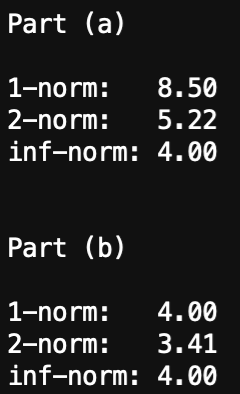
\includegraphics[width=0.3\textwidth]{prob5.png} 
\end{center}



\prob{6}{
Determine SVDs of the following matrices by hand calculation and MATLAB.
}

(a) $\begin{pmatrix}
    3 & 0 \\
    0 & -2
\end{pmatrix}
$

First, we solve the eigenproblem for $A^{\rm T}A$, where we denote the matrix above as $A$.
\begin{eqnarray}
    \label{eq:AT-A_6}
    A^{\rm T}A = \begin{pmatrix}9 & 0\\0 & 4\end{pmatrix} 
.\end{eqnarray}
Then the characteristic equation is
\begin{eqnarray}
    \label{eq:char-eq_6}
    \lambda^{2} - 13 \lambda + 36 = 0 \Rightarrow \lambda \in \{4,9\}
.\end{eqnarray}
Now, we find the eigenvectors of $A^{\rm T}A$ for each eigenvalue $x$, which are trivial to read off since $A^{\rm T}A$ is diagonal:
\begin{align}
    \label{eq:corresponding-eigvec_6}
    &\lambda = 9: \quad x = \begin{pmatrix} 1 & 0 \end{pmatrix}^{\rm T} \\
    &\lambda = 4: \quad x = \begin{pmatrix} 0 & 1 \end{pmatrix}^{\rm T}
.\end{align}
Hence
\begin{eqnarray}
    \label{eq:Sig-V_6}
    \eqbox{
    \Sigma = \begin{pmatrix}
        3 & 0 \\
        0 & 2 
    \end{pmatrix}
    \quad
    V = \id_{2 \times 2} 
}
.\end{eqnarray}
Finally, we find the columns of $U$ by solving $u_{j} = Av_{j}/\sigma_{j}$ for $j = 1,2$:
\begin{align}
    \label{eq:U-vecs_6}
    u_{1} &= \frac{1}{3}\begin{pmatrix}
        3 & 0 \\
        0 & -2 
    \end{pmatrix}
    \begin{pmatrix}
    1 \\ 0
    \end{pmatrix}
    = 1  \\
    u_{2} &= \frac{1}{2}\begin{pmatrix}
        3 & 0 \\
        0 & -2
    \end{pmatrix}
    \begin{pmatrix}
    0 & -1   
    \end{pmatrix}
    = -1
,\end{align}
which means
\begin{eqnarray}
    \label{eq:U_6}
    \eqbox{
    U = \begin{pmatrix}
        1 & 0 \\
        0 & -1
    \end{pmatrix}
}
.\end{eqnarray}

(b) $
\begin{pmatrix}
    0 & 2 \\
    0 & 0 \\
    0 & 0 \\
    0 & 0
\end{pmatrix}
$

We perform the SVD in the same way as above.
First, we diagonalize $A^{\rm T}A = \begin{pmatrix}0 & 0 \\ 0 & 4\end{pmatrix}$.
Incidentally, $A^{\rm T}A$ is already diagonal, so we can read off its eigenvalues and eigenvectors directly: $\lambda \in \{ 0,4 \} $ with corresponding eigenvectors $\begin{pmatrix}1 & 0\end{pmatrix}^{\rm T}$ and $\begin{pmatrix}0 & 1\end{pmatrix}^{\rm T}$.
Now we can write down our matrices for the SVD as follows
\begin{eqnarray}
    \label{eq:SVD-matrices}
    \eqbox{
    U = 
    \begin{pmatrix}
        1 & 0 & 0 & 0 \\
        0 & 0 & 0 & 0 \\
        0 & 0 & 0 & 0 \\
        0 & 0 & 0 & 0 
    \end{pmatrix}
    \quad
    \Sigma = 
    \begin{pmatrix}
        2 & 0 \\
        0 & 0 \\
        0 & 0 \\
        0 & 0 
    \end{pmatrix}
    \quad
    V = 
    \begin{pmatrix}
        0 & 1 \\
        1 & 0
    \end{pmatrix}
    }
.\end{eqnarray}

The code for parts (a) and (b) of this problem is shown below along with a screenshot of the output:

\inputpython{prob6.py}
\begin{center}
    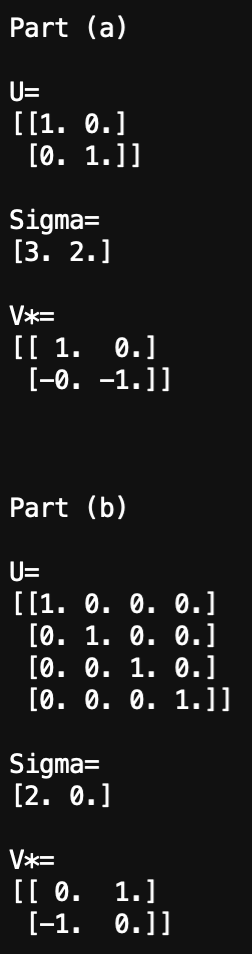
\includegraphics[width=0.3\textwidth]{prob6.png}
\end{center}


\end{document}
